\section{Non-Multi-Fact Reasoning}

\subsection{Characterizing Non-Multi-fact Reasoning}

There can be various kinds of biases and artifacts present in the dataset that could pave shortcuts for models to predict the property correctly without the intended reasoning. In this work, we discuss about one kind of artifact (or bias) based reasoning that deals with \textit{multi-fact}edness of reasoning on multi-fact reasoning task. \harsh{I think this clarifies that in what we mean by non-multi-fact reasoning, the \textit{non} is on \textit{multi-fact}edness and not the \textit{reasoning}}

In a multi-fact QA dataset, the intended reasoning is to aggregate and synthesis together information from \textit{all} the supporting facts to arrive at the predicted conclusion. So we define non-multi-fact reasoning bias or artifact as the extent to which the information accessible by the model is present in the dataset to correctly predict all the task labels, without any non-trivial synthesis of information from \textit{all} the supporting facts.

Concretely, in a multi-fact QA dataset {\it D} with desired prediction property {\it P}, the extent of non-multi-fact reasoning bias accessible by the model {\it M} is measured by the maximum fraction of questions in {\it D} in which following conditions hold:

\begin{itemize}
    \item \textbf{Base condition:} model can predict exactly correctly {\it P} for the question.
    \item \textbf{NMF condition:} there exists at least one bi-partition of the supporting facts, such that without any \textit{non-trivial} synthesis of the two parts of the bi-partition among the context facts, the model can predict exactly correctly {\it P} for the question.
\end{itemize}

% \noindent \textbf{NMF Condition:} there exists at least one bi-partition of the supporting facts, such that without any \textit{non-trivial} synthesis of the two parts of the bi-partition among the context facts, the model can predict exactly correctly {\it P} for the question.

In practice, we probe NMF condition based on a re-written condition:

\noindent \textbf{NMF Condition:} there exists at least one bi-partition of the supporting facts, such that model predictions for property {\it P} of two parts of the bi-partitions (each part corresponds to the same context except without that supporting facts from that part) can be trivially combined together to predict exactly correctly {\it P} for the question.

\begin{figure}[t]
    \centering
	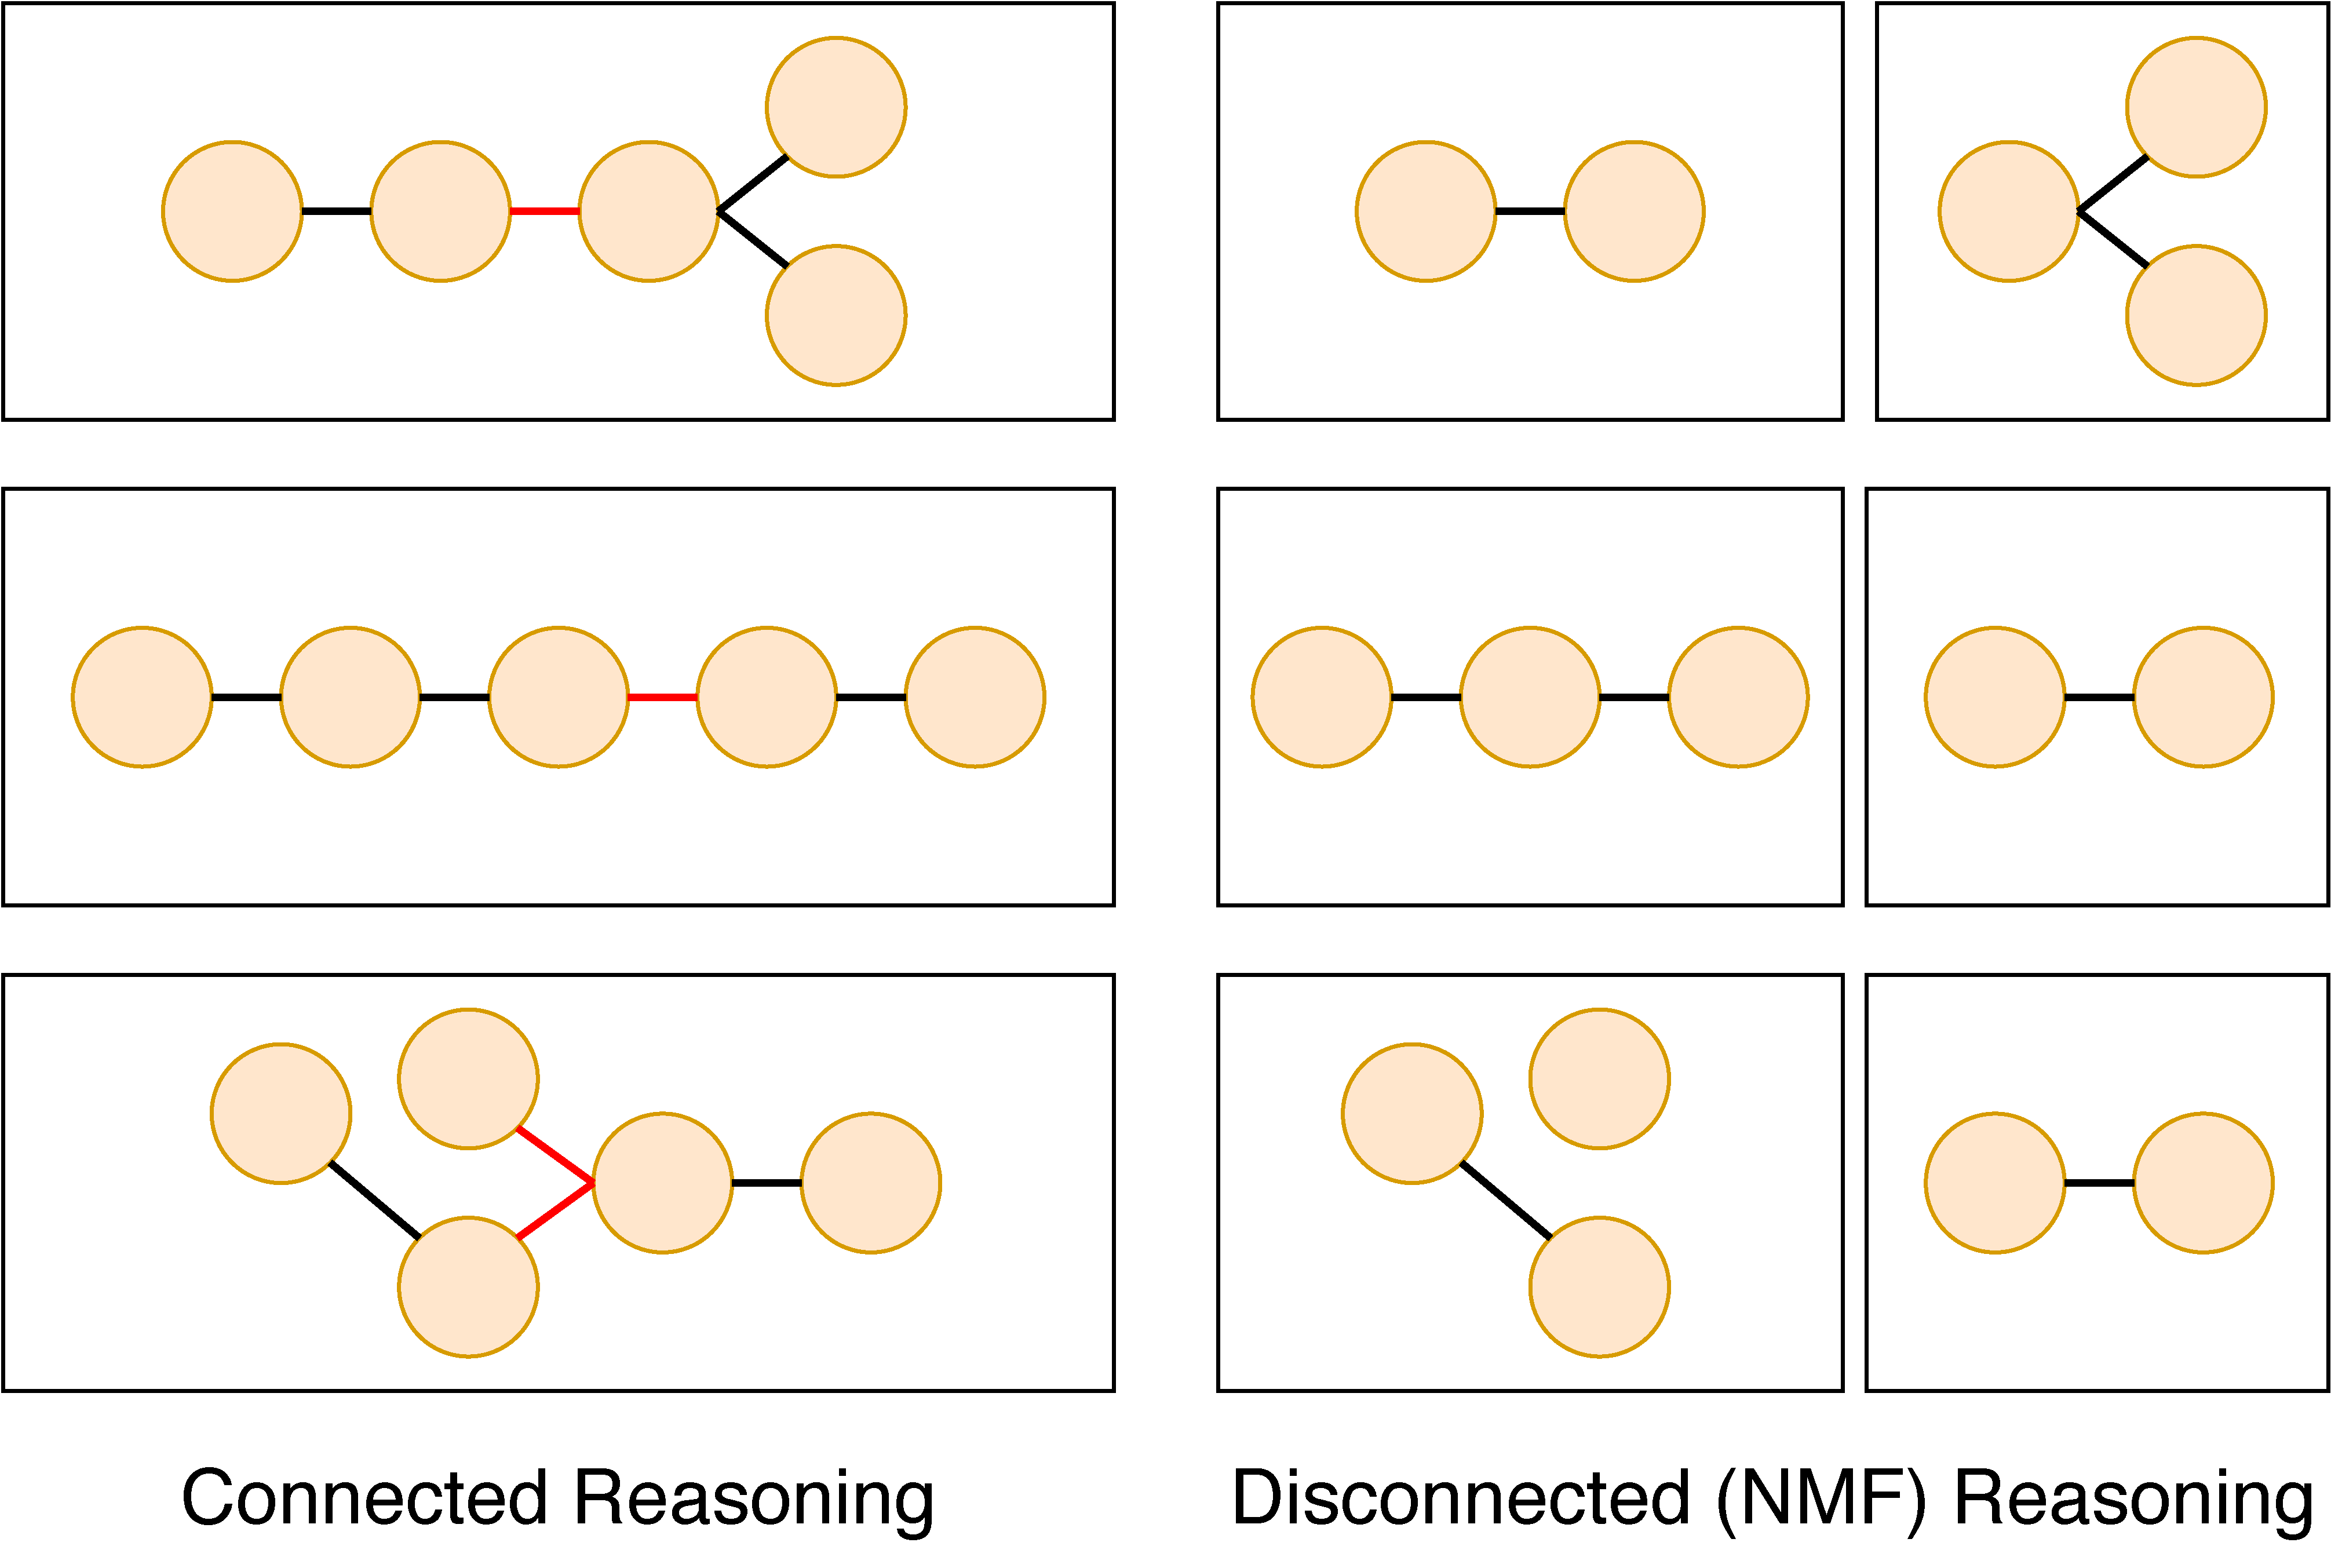
\includegraphics[width=0.45\textwidth]{images/factored-graph-v2}
	\caption{TODO: Explain }
	\label{fig:intro}
\end{figure}

Formally, for each property $P$, we want to check if the following is possible for some simple aggregation function $f_s$:

\begin{align}
     & P_r(P | (Q; F_{s_1} + F_{s_1} + F_d)) \nonumber  \\
    =& f_{s}\big(P_r(P | (Q; F_{s_1} + F_d)), P_r(P | (Q; F_{s_2} + F_d)) \big) \nonumber 
\end{align}

\harsh{Maybe the whole explanation of NMF reasoning can be explained in terms of factorization of joint probability distribution. Thoughts?}

We say that the multi-fact dataset property $P$ can be hacked by model $M$ with only non-multi-fact reasoning based on the maximum number of questions in which \textbf{Base} and \textbf{NMF} conditions hold.

We say that the amount of non-multi-fact reasoning a model could do as the fraction of maximum number of questions in which \textbf{Base} and \textbf{NMF} conditions hold to the maximum number of questions in which \textbf{Base} condition holds.

In \textbf{NMF} condition, we have used a notion of \textit{trivial combination}. Since the properties take various forms like span, set or list of items to name a few, it's difficult to define trivial combination in a completely property agnostic way. We instantiate the NMF condition for each property separately.


\subsubsection{Answer Prediction}

For input instance $(Q, C)$, the model should output answer $A$. But if there is a partition $(F_{s1}, F_{s2})$ of $F_s$ such that the model also correctly outputs $A$ on at least one of $(Q, F_{s1} + F_d)$ and $(Q, F_{s2} + F_d)$ as input, then we can say it is has information to do non-multi-fact reasoning for answer prediction.

\subsubsection{Supporting Fact Prediction}

For input instance $(Q, C)$, the model should output $L_s = F_s$. But if there is a partition $(F_{s1}, F_{s2})$ of $F_s$ such that the model also correctly outputs $F_{s1}$ in $(Q, F_{s1} + F_d)$ and $F_{s2}$ in $(Q, F_{s2} + F_d)$ as input, then we say it is has information to do non-multi-fact reasoning for supporting facts prediction.

\subsubsection{Support Sufficiency Prediction}

For input instance $(Q, C)$, the model should output $L_c = 0$ for \textit{every} variation of insufficient instance and sufficient instance for the question $Q$. But for \textit{every} subset of the supporting facts if it can differentiate between the presence and absence of the supporting facts among the distracting facts in the context, then it can decide $L_c$ labels for every variation without any synthesis of information from the supporting facts.

To see this, consider sufficient instance $(Q, F_s + F_d'; L_C=1)$ and a partition of $F_s$ as $F_{s1}$ and $F_{s2}$, and the corresponding insufficient instances $(Q, F_{s1} + F_{r1} + F_d'; L_C=0)$ and $(Q, F_{s2} + F_{r2} + F_d'; L_C=0)$. If the model can differentiate the inputs $(Q, F_{s1} + F_d')$ vs $(Q, + F_{r1} + F_d')$ and $(Q, F_{s2} + F_d')$ vs $(Q, F_{r2} + F_d')$, then it can predict the sufficiency labels ($L_C$) of \textit{all} three instance variations without any inter-dependence (\harsh{interaction might be confusing word here}) of supporting facts in $F_{s1}$ and $F_{s2}$. The same can be extrapolated for all partitions of $F_s$ and so we can say that if model can distinguish the presence vs absence of \textit{every} subset of $F_s$, then we can say it has information to do non-multi-fact reasoning for support sufficiency prediction.


\eat{
    % \begin{enumerate}
    %     \item model can predict exactly correctly {\it P} for the question.
    %     \item there exists at least one bi-partition of the supporting facts, such that without any \textit{non-trivial} synthesis of the two parts of the bi-partition among the context facts, the model can predict exactly correctly {\it P} for the question.
    %     % there exists at least one bi-partition of the supporting facts, such that model predictions of individual parts of the bi-partitions for the desirable predictables can be trivially combined together to obtain the correct desirable predictables of the question.
    % \end{enumerate}

    % If the intended multi-fact reasoning is $n$-fact reasoning where the information from known $n$ supporting facts need to be synthesised together to arrive at a conclusion, we often find dataset artifacts can allow models to arrive at the right conclusion without any non-trivial synthesis (or even usage) of information from \textit{all} the $n$ supporting facts. We call such artifact based reasoning on the dataset non-multi-hop reasoning.
    
    % Although ability to predict such properties is a desirable one, it does not imply good reasoning owing to various biases and artifacts present in the dataset that pave shortcuts for models to predict correctly the correct property without the intended reasoning.
    
    % Following the broad definition of multi-hop reasoning, it is difficult to probe whether an entity is really capable of good multi-hop reasoning or not in that we don’t have a clear definition of ``meaningful” composition or aggregation. But we can check if the information accessible by the model is present in the dataset to correctly predict all the task labels, without any non-trivial composition from the supporting facts.
    
    % We consider that a model is doing non-multi-hop reasoning if it
    
    % \begin{enumerate}
    %     \item correctly predicts all desirable predictable properties (labels) for the question.
    %     \item there exists at least one bi-partition of the supporting facts, such that without any non-trivial composition or aggregation of the two parts of supporting facts, all desirable predictable properties for the question can be correctly predicted.
    %     % there exists at least one bi-partition of the supporting facts, such that model predictions of individual parts of the bi-partitions for the desirable predictables can be trivially combined together to obtain the correct desirable predictables of the question.
    % \end{enumerate}

}


\subsection{Measuring Non-Multi-fact Reasoning}

We describe now a way to automatically generate a probing dataset training and evaluating a model on which can directly give us the extent of non-multi-fact reasoning possible on a dataset by a model for predicting a given property. 

Training and evaluating a model {\it M} on original dataset task $D_{base}$ in predicting property $P$ lets us know the maximum number of questions in which model can satisfy the \textbf{base} condition. We create a transformation of the dataset task $D_{nmf}$ training and evaluating model architecture {\it M} on it let us know the maximum number of questions in which model can satisfy both \textbf{base} and \textbf{NMF} condition. The accuracy on $D_{nmf}$ can be understood as the extent of score that the model architecture M could have achieved on D via only non-multi-fact reasoning. 

% Our effort with non-multi-fact reasoning is to capture as much non-multi-hop reasoning as possible in a question-agnostic and a model-agnostic way. So we do allow the non-multi-hop reasoning to have compositions among multiple supporting facts as long as there's a clear partition. For example in a 5 multi-hop dataset, a model considered to bad reasoning even if locally integrates first 2 facts and second 3 facts which are combined trivially. This is because there's no non-trivial dependence on second part of this partition based on the first and vice-versa.

Now, we describe the procedure to make this transformation for each of the three desirable properties. Consider a dataset with question $Q$, answer $A$, supporting fact $F_s$, other set of distractor facts $F_d$. Let one partition of supporting facts $F_s$ be $F_{s_1}$ and $F_{s_2}$. Sample $|F_s| + |F_d| - |F_{s_1}|$ number of facts from $F_d$ to get $F_{r_1}$, sample $|F_s| + |F_d| - |F_{s_2}|$ number of facts from remaining $F_d$ to get $F_{r_2}$ and let the remaining other facts from $F_d$ be $F_d'$.

\subsubsection{Answer Prediction}

We transform the instance $(Q, F_s + F_d; L_a=A)$ of $D_{base}$ to instances $D_{nmf}$ as:

\begin{enumerate}[noitemsep]
    \item $(Q, F_s + F_d; L_a=A)$
    \item $(Q, F_{s_1} + F_d; L_a=A)$
    \item $(Q, F_{s_2} + F_d; L_a=A)$
\end{enumerate}

\harsh{TODO: Need a notation or way of formally explaining all intersections and unions (for all possible partitions) as in \href{https://docs.google.com/presentation/d/1CVWAJYPcGMKomNW-g3wBhrD05Ad0u-I0I1yaDCPt7pc/edit#slide=id.g71e43d5645_0_339}{here}}

The model gets a point $Q$ only if it gets instance 1 and any of 2 and 3 right. The instances 2 and 3 are repeated for all bipartitions of set $F_s$, such that both parts are non-empty. If a model gets instance 2 and 3 right, the model has the information required to get instance 1 right without any non-trivial composition of facts in $F_{s_1}$ and $F_{s_2}$. The model needs to make predictions on these instances independent of each other.

\eat{
    % So for answer prediction, we consider that a model is doing non-multi-hop reasoning if it
    % \begin{enumerate}
    %     \item correctly identifies the answer for the question.
    %     \item there exists at least one bi-partition of the supporting facts, such that model identifies the answer in at least one of the two parts.
    % \end{enumerate}
}

\subsubsection{Supporting Facts Prediction}

Given an instance $(Q, F_s + F_d, L_c=F_s)$ of $D_{base}$, let $\mathcal{P}_s$ denote the set of all bi-partitions of $F_s$.\footnote{$\mathcal{P}_s = \{(F_{s_1}, F_{s_2}) \mid F_{s_1} \cup F_{s_2} = F_s, F_{s_1} \cap F_{s_2} = \phi\}$} We transform this instance into $|\mathcal{P}|$ grouped instances in $D_{nmf}$, where the bipartition $\rho = (F_{s_1}, F_{s_2}) \in \mathcal{P}$ corresponds to the following grouped instance $d_\rho$:

% We transform the instance $(Q, F_s + F_d, L_c=F_s)$ of $D_{base}$ to instances $D_{nmf}$ as:

\begin{enumerate}[noitemsep]
    \item $(Q, F_s + F_d; L_s=F_s)$
    \item $(Q, F_{s_1} + F_d; L_s=F_{s_1})$
    \item $(Q, F_{s_2} + F_d; L_s=F_{s_2})$
\end{enumerate}

The model gets a point only if it is correct on instances 1, 2 and 3 for \emph{some} partition $\rho$.
% The instances 2 and 3 are repeated for all bipartitions of set $F_s$, such that both parts are non-empty.
If a model gets instance 2 and 3 right, the model has the information required to get instance 1 right without any non-trivial composition of facts in $F_{s_1}$ and $F_{s_2}$. The model needs to make predictions on these instances independent of each other.

\eat{
    % So for relevance prediction, we consider that a model is doing non-multi-hop reasoning if it
    
    % \begin{enumerate}
    %     \item Correctly identifies all supporting facts for the question.
    %     \item there exists at least one bi-partition of the supporting facts, such that model identifies the answer in at least one of the two parts, where 
    %      identifying independently a subset means model can identify ALL facts of the subset among a mix with distractor ($F_o$) facts, without rest of the supporting facts.
    % \end{enumerate}
}

\subsubsection{Support Sufficiency Prediction}

We transform the following question group of instances:

\begin{enumerate}[noitemsep]
    \item $(Q, F_s + F_d'; L_c=1)$
    \item $(Q, F_{s_1} + F_{r_1} + F_d'; L_c=0)$
    \item $(Q, F_{s_2} + F_{r_2} + F_d'; L_c=0)$
\end{enumerate}

\noindent of $D_{base}$ to instances $D_{nmf}$ as

\begin{enumerate}[noitemsep]
    \item $(Q, F_s + F_d'; L_c=1)$
    \item $(Q, F_{s_1} + F_d'; L_c=0)$
    \item $(Q, F_{s_2} + F_d'; L_c=0)$
    \item $(Q, F_{r_1} + F_{r_2} + F_d'; L_c=-1)$
\end{enumerate}

Note that the semantics of class label $L_C$ are different in $D_{base}$ and $D_{nmf}$. The model can separate the $L_c=1$ vs $L_c=0$ in without any interaction or dependence between $F_{s_1}$ and $F_{s_2}$, if model can solve the following binary classification task:

\begin{enumerate}[noitemsep]
    \item $(Q, F_{s_1} + F_d', L_c=0)$
    \item $(Q, F_{r_1} + F_d', L_c=-1)$
    \item $(Q, F_{s_2} + F_d', L_c=0)$
    \item $(Q, F_{r_2} + F_d', L_c=-1)$
\end{enumerate}

Note that $F_{r_1}$ and $F_{r_2}$ are randomly sampled from $F_d$ meaning that they both come from the same distribution as distractor facts. So the model can hack the sufficiency of all variations of the question without interaction or composition between the two parts of the supporting facts partition if model can individually identify the presence vs absence of individual parts among the set of distractor facts.

\eat{
    % So for sufficiency prediction, we consider that a model is doing non-multi-hop reasoning if it
    
    % \begin{enumerate}
    %     \item Correctly identifies sufficiency for all 3 variations from all bi-partition of supporting facts for the question.
    %     \item For all bi-partitions of the supporting facts, model independently identifies presence or absence of both parts (subsets) of the bi-partition among the set of distractor facts.
    % \end{enumerate}
}
